
%(BEGIN_QUESTION)
% Copyright 2004, Tony R. Kuphaldt, released under the Creative Commons Attribution License (v 1.0)
% This means you may do almost anything with this work of mine, so long as you give me proper credit

Calculate the load current and load voltage in this transformer circuit:

$$\includegraphics[width=15.5cm]{i04756x01.eps}$$

$I_{load}$ = \hskip 80pt $V_{load}$ =

\vskip 20pt \vbox{\hrule \hbox{\strut \vrule{} {\bf Suggestions for Socratic discussion} \vrule} \hrule}

\begin{itemize}
\item{} How do the input and output {\it power} levels in a transformer circuit compare?  Voltages and currents may be stepped up and down, but what about watts?  Explain why.
\end{itemize}

\underbar{file i04756}
%(END_QUESTION)





%(BEGIN_ANSWER)

$I_{load}$ = 23.77 mA \hskip 80pt $V_{load}$ = 8.318 V

%(END_ANSWER)





%(BEGIN_NOTES)

Most transformer problems are nothing more than ratios, but some students find ratios difficult to handle.  Questions such as this are great for having students come up to the board in the front of the classroom and demonstrating how they obtained the results.

%INDEX% Electronics review: AC transformer circuit

%(END_NOTES)


